\let\negmedspace\undefined
\let\negthickspace\undefined
\documentclass[journal]{IEEEtran}
\usepackage[a5paper, margin=10mm, onecolumn]{geometry}
%\usepackage{lmodern} % Ensure lmodern is loaded for pdflatex
\usepackage{tfrupee} % Include tfrupee package

\setlength{\headheight}{1cm} % Set the height of the header box
\setlength{\headsep}{0mm}     % Set the distance between the header box and the top of the text

\usepackage{gvv-book}
\usepackage{gvv}
\usepackage{cite}
\usepackage{amsmath,amssymb,amsfonts,amsthm}
\usepackage{algorithmic}
\usepackage{graphicx}
\usepackage{textcomp}
\usepackage{xcolor}
\usepackage{txfonts}
\usepackage{listings}
\usepackage{enumitem}
\usepackage{mathtools}
\usepackage{gensymb}
\usepackage{comment}
\usepackage[breaklinks=true]{hyperref}
\usepackage{tkz-euclide} 
\usepackage{listings}
% \usepackage{gvv}                                        
\def\inputGnumericTable{}                                 
\usepackage[latin1]{inputenc}                                
\usepackage{color}                                            
\usepackage{array}                                            
\usepackage{longtable}                                       
\usepackage{calc}                                             
\usepackage{multirow}                                         
\usepackage{hhline}                                           
\usepackage{ifthen}                                           
\usepackage{lscape}
\usepackage{xr}
\externaldocument{/home/homa/Desktop/matgeo/main}
\begin{document}

\bibliographystyle{IEEEtran}
\vspace{3cm}

\title{3-3.3-8}
\author{EE24BTECH11062 - Homa Harshitha Vuddanti
}
% \maketitle
% \newpage
% \bigskip
{\let\newpage\relax\maketitle}

\renewcommand{\thefigure}{\theenumi}
\renewcommand{\thetable}{\theenumi}
\setlength{\intextsep}{10pt} % Space between text and floats


\numberwithin{equation}{enumi}
\numberwithin{figure}{enumi}
\renewcommand{\thetable}{\theenumi}


\textbf{Question}:\\
Construct a triangle $ABC$ with side $BC = 7 cm, \angle{B}=45\degree , \angle{A}=105\degree$.   
\\
\textbf{Solution: }\\
Given,\\
\begin{table}[h!]    
  \centering
  \begin{tabular}[12pt]{ |c| c|}
    \hline
    \textbf{Variable} & \textbf{Description}\\ 
    \hline
    $a$ & $7cm$\\
    \hline 
    $\angle{B}$ & $45\degree$\\
    \hline
    $\angle{A}$ & $105\degree$\\
    \hline
    \end{tabular}




  \caption{Given variables}
  \label{3-3.3-8-table}
\end{table}

By angle sum property,
\begin{align}
    \angle{A}+\angle{B}+\angle{C}&=180\degree\\
    \angle{C}&=180\degree-\brak{45\degree+105\degree}\\
    \angle{C}&=30\degree\label{3-3.3-8-3}
\end{align}
Using Sine formula, in $\triangle ABC$,
\begin{align}
    \frac{a}{sin A}=\frac{b}{sin B}=\frac{c}{sin C}
\end{align}
 \begin{align}
    b&=\frac{sin B}{sin A}a\\
    b&=\frac{sin \frac{\pi}{4}}{sin \frac{7\pi}{12}}7cm\\
    b&=\frac{14}{\sqrt{3}+1}\label{3-3.3-8-4}\\
    c&=\frac{sin C}{sin A}a\\
    c&=\frac{sin \frac{\pi}{6}}{sin \frac{7\pi}{12}}7cm\\
    c&=\frac{14}{\sqrt{2}\brak{\sqrt{3}+1}}\label{3-3.3-8-5}
\end{align}
 From equations \eqref{3-3.3-8-4}, \eqref{3-3.3-8-5} and  
 \eqref{eq:9/11/2/1},
\begin{align}
\vec{A}&=c\myvec{cos B\\ sin B}=\frac{14}{\sqrt{2}\brak{\sqrt{3}+1}}\myvec{cos \frac{\pi}{4}\\ sin \frac{\pi}{4}}\\
\vec{B}&=0\\
\vec{C}&=\myvec{a \\ 0}=\myvec{7\\0}
\end{align}
\begin{figure}[h!]
   \centering
   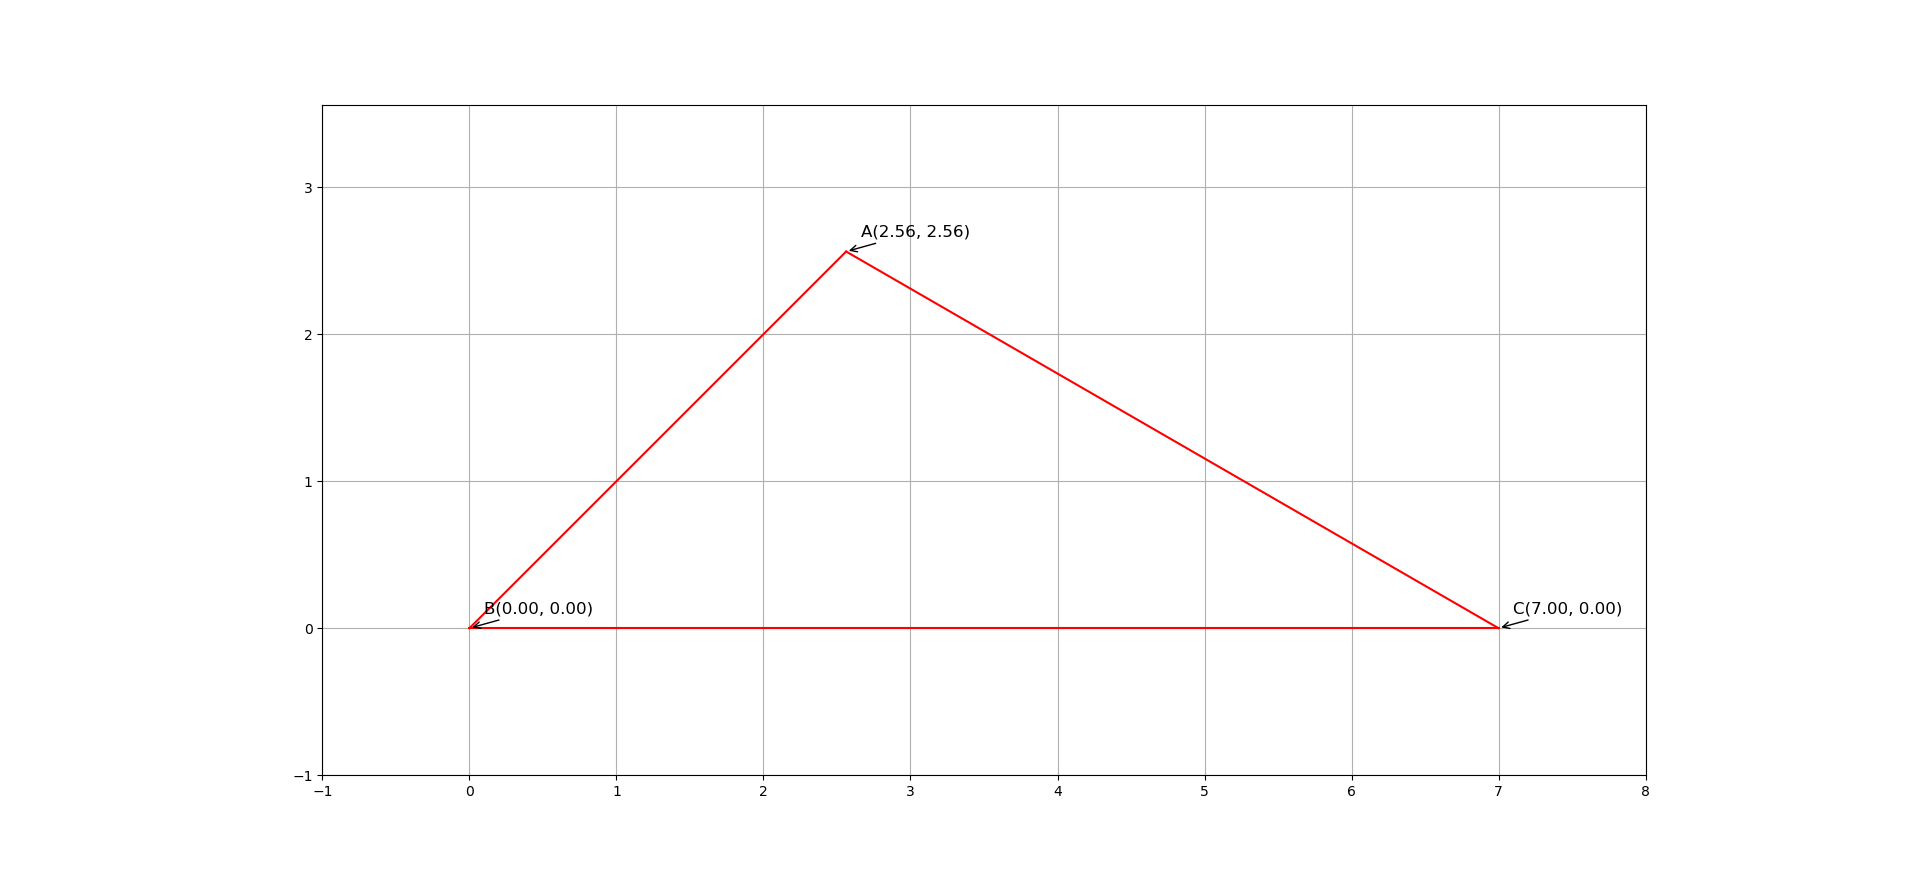
\includegraphics[width=1.1\columnwidth]{Figs/Figure_1.png}
   \caption{Plot}
   \label{3-3.3-8-Figure}
\end{figure}
\end{document}  






